\documentclass[twoside,11pt]{article}
\usepackage[slovene]{babel}
\usepackage[utf8]{inputenc}
\usepackage{graphicx}
\usepackage[frame]{matrika}
\usepackage{mathtools}
\usepackage{epstopdf}
\usepackage{units}
\usepackage{url}
\usepackage{amsfonts}
\usepackage{amsmath}
\usepackage{tikz}

\usetikzlibrary{arrows.meta}

\begin{document}

\MAT{1}{11}{2024}
\naslov{Stohastični abakus}

\avtor{Luka Houška}

\institucija{Fakulteta za matematiko in fiziko \\ Univerza v Ljubljani}

\date{23.10.2023}

\klasifikacija{~} 
\izvlecek{V članku je podrobno predstavljen stohastični abakus, kako algoritem deluje in zakaj deluje. S pomočjo stohastičnega abakusa so analizirane igre ,,podajanja evra`` na različnih grafih, kar razkrije naravno povezavo s Fibonaccijevimi števili.}
\title{Probabilistic abacus}
\abstract{The article presents stochastic abacus in detail, how the algorithm works and why it works. Using the stochastic abacus, pass-the-buck games are analyzed on various graphs, revealing a natural connection with the    Fibonacci numbers.}

\glava
\baselineskip=14.5pt

\smallskip

\section{Uvod}
Igra ,,podajanja evra`` se začne z $n$ igralci postavljenimi kot vozlišča grafa. En igralec ima v roki evro. Igra se igra izmenično, kjer v vsakem koraku igralec, ki v roki drži evro, odvisno od naključja zmaga ali pa poda evro enemu od igralcev na sosednjih vozliščih. Če ima vozlišče trenutnega igralca stopnjo $d$, je vsak od $d + 1$ izidov, torej da zmaga ali poda evro enemu od sosedov, enako verjeten. Pri igri bomo uporabljali koncept ,,izstreljevanja žetonov`` (angl. \emph{chip firing}), ki ga je kot sredstvo za poučevanje verjetnosti osnovnošolcem razvil oče stohastičnega abakusa Arthur Engel.
Osnovna ideja izstreljevanja žetonov je preprosta. Če imamo podan graf, si predstavljamo, da v vozlišča dodamo nekaj žetonov. Če je število žetonov v vozlišču $v$ večje ali enako kot stopnja $v$, potem lahko žetone \emph{izstrelimo} iz $v$ tako, da do vsakega soseda $v$ po povezavi pošljemo en žeton. Število žetonov v vozlišču $v$ se po izstrelitvi zmanjša za stopnjo $v$, vsakemu od sosednjih vozlišč $v$ pa se število žetonov poveča za ena. 
Koncept izstreljevanja žetonov bomo implementirali na \emph{usmerjene grafe}, kjer bo izstrelitev iz vozlišča $v$ pomenila, da po vsaki izhodni povezavi iz $v$ pošljemo en žeton. Natančneje, usmerjeni graf bo prehodni graf za absorbirajočo Markovsko verigo, ki ustreza igri podajanja evra. Naša naloga je, da natančno predstavimo Engelov originalni koncept, ki uporablja izstreljevanje žetonov kot sredstvo za računanje verjetnosti in pričakovanih vrednosti. Naš prvi korak je spoznati Engelov algoritem.

\section{Stohastični abakus}
V začetku 1970-ih je Engel razvil svoj algoritem, ki ga je kasneje poimenoval stohastični abakus, saj premikanje žetonov po povezavah v grafu za namen računanja spominja na tradicionalni abakus.
\indent Predpostavimo, da imamo tako časovno diskretno absorbirajočo Markovsko verigo s končnim številom stanj, da so vse prehodne verjetnosti racionalna števila. Predstavimo jo z usmerjenim grafom, kjer so stanja vozlišča in usmerjena povezava med vozliščema $u$ in $v$ obstaja natanko tedaj, ko je verjetnost direktnega prehoda iz $u$ v $v$ pozitivna. 
Natančneje, če je $q$ najmanjši skupni imenovalec vseh prehodnih verjetnosti iz stanja $u$ in je verjetnost prehoda iz $u$ v $v$ enaka $p/q$, potem postavimo p usmerjenih povezav iz $u$ v $v$. Če to naredimo za vse sosede $u$, je izhodna stopnja $u$ enaka $q$. Zato se prehodne verjetnosti lahko razberejo iz usmerjenega grafa brez uporabe uteži na povezavah. 
Uporabljali bomo izraza \emph{notranja vozlišča} za minljiva stanja in \emph{končna vozlišča} za absorbirajoča stanja. \\
\indent Ideja algoritma je, da začnemo s praznimi vozlišči in dodajamo žetone v izbrano (minljivo) začetno stanje, ki ga bomo poimenovali začetno vozlišče. Ko je v začetnem vozlišču dovolj žetonov, izstrelimo žetone iz njega tako, da po povezavah do sosednjih vozlišč pošljemo žetone v razmerju, ki odražajo prehodne verjetnosti. Ponavljamo postopek dodajanja in izstreljevanja žetonov, dokler nima vsak od sosedov dovolj žetonov, da izstrelimo te, itn. Predstavljajmo si, da ponavljamo postopek dodajanja in izstrelitev žetonov in
da je na neki točki število žetonov na notranjih vozliščih enako začetnemu. Engel je utemeljil, da je v tem trenutku število žetonov v končnih vozliščih proporcionalno verjetnostim, da pridemo v absorbirajoče stanje, ki ga to vozlišče predstavlja, saj premikanje žetonov po grafu upošteva prehodne verjetnosti. %Če smo bolj natančni: če ima končno vozlišče $k$ žetonov in je število vseh dodanih žetonov v začetno vozlišče $c$, potem je verjetnost, da pridemo v to absorbirajoče stanje iz začetnega stanja enaka $k/c$. Ker smo ustvarili periodičen proces; če dodajamo žetone v začetno vozlišče in ponovimo celoten postopek, bo končna razporeditev žetonov v končnih vozliščih enaka, saj more po zakonu o velikih številih biti v razmerju z verjetnostmi. Ker pa je proces periodičen je ena iteracija dovolj, da odkrijemo pravilna razmerja žetonov v končnih vozliščih. \\
\newline 
\indent S tem algoritmom sta dva potencialna problema, ki ju je Engel razrešil. Prvič, ni težko pokazati, da je vrstni red izstrelitev žetonov nepomemben. To pomeni, da je sproščanje sistema, tj. izstrelitev žetonov iz vseh primernih vozlišč, dobro definirano. Drugič, treba je ugotoviti, kako prvotno postaviti žetone na notranjih vozliščih, da imamo zagotovljeno, da se bo sistem vrnil v to razporeditev. To nam pove trditev \ref{končnost}.  

\begin{definicija}\label{kritična razporeditev}
    \textbf{Kritična razporeditev} žetonov je začetna razporeditev žetonov, za katero velja, da v začetno vozlišče $u$ z izhodno stopnjo $d$ naložimo $d$ žetonov, v ostala notranja vozlišča $v$ z izhodno stopnjo $d_{v}$ naložimo $d_{v} - 1$ žetonov, končna vozlišča pa pustimo prazna.
\end{definicija}

\begin{trditev}\label{končnost}
    Če algoritem začnemo s kritično razporeditvijo žetonov, se bo ta ponovila po končnem številu korakov.
\end{trditev}

\noindent {\em Dokaz:\/} Zapišimo prehodne verjetnosti kot $p_{ij} = \frac{r_{ij}}{r_{i}},\; r_{ij}, r_{i}\in \mathbb{N}$. Potezo, kjer iz vozlišča $i$ izstrelimo $r_{ij}$ žetonov v vozlišče $j$ za vsak $j$, bomo poimenovali poteza \emph{tipa 1}. Potezo, kjer vozlišču $u$ dodamo žeton, bomo poimenovali poteza \emph{tipa 2}. Izberimo še neko minljivo stanje $u$, ki bo naše začetno vozlišče. Začnimo z neko začetno razporeditvijo žetonov, ki je manjša ali enaka kot kritična, torej vsakemu vozlišču dodamo manj ali enako žetonov kot bi jih imel v kritični razporeditvi. Nadaljujemo z algoritmom, dokler se neka razporeditev žetonov na notranjih vozliščih $b_{1},b_{2},\ldots,b_{r}$ ne ponovi. Takšna zaporeditev zagotovo obstaja, saj imamo končno število vozlišč, število žetonov na notranjih vozliščih ob istem času pa je navzgor omejeno z vsoto vseh izstopnih stopenj, torej imamo omejeno število različnih razporeditev žetonov na notranjih vozliščih. Vzemimo to razporeditev $b_{1},b_{2},\ldots,b_{r}$ za začetno. Lahko predpostavimo, da je $b_{i}<r_{i}$ za $i \neq u$ in $b_{u} = r_{u}$. Izberimo za to razporeditev zelene žetone. Nato dodajmo rdeče žetone, da razporeditev dopolnimo do kritične. Nato nadaljujemo z enakim zaporedjem potez, vendar uporabljamo samo zelene žetone. Ko se bo naša začetna razporeditev ponovila, bomo spet imeli kritično razporeditev, saj se rdečih žetonov nismo dotaknili. Poimenujmo ta modificiran postopek \emph{metoda A}. 
Predpostavimo, da smo v metodi A v vozlišče $u$ dodali $m$ žetonov. Poglejmo zdaj še drugo metodo, ki jo bomo poimenovali \emph{metoda B}. V metodi B bomo začeli s kritično razporeditvijo žetonov in izvajali algoritem, dokler ne dodamo $m$ žetonov in ne moremo narediti več nobene poteze tipa 1. Pokazali bomo, da obe metodi pripeljeta do enake končne razporeditve žetonov. Ker vemo, da je končna razporeditev v metodi A kritična, bo enako veljalo tudi za metodo B. \newline
\indent Naj bo $e_{1},e_{2},\ldots,e_{n}$ zaporedje potez, ki smo jih naredili v metodi A in naj bo $f_{1},f_{2},\ldots,f_{v}$ zaporedje potez v metodi B. Potezi $e_{1}$ in $f_{1}$ sta enaki, saj v obeh primerih izstrelimo $r_{u}$ žetonov iz vozlišča $u$. Z indukcijo bomo dokazali, da se vse poteze $e_{i}, i \in [n], $ pojavijo nekje v zaporedju $\{ f_{j}\} _{j\in [v] }$. Predpostavimo, da smo za poteze $e_{1},e_{2},\ldots,e_{k}$ našli enake poteze $f_{i_1},f_{i_2},\ldots,f_{i_k}$. Poglejmo potezo $e_{k+1}$. Če je to poteza tipa 2, mora obstajati enaka poteza $f_{i_{k+1}}$, saj v obeh metodah naredimo $m$ takšnih potez.
Predpostavimo sedaj, da je $e_{k+1}$ poteza tipa 1, recimo, da izstrelimo $r_{t}$ žetonov iz vozlišča $t$. Če obstaja taka poteza $f_{i_{k+1}}$, torej da izstrelimo $r_{t}$ žetonov iz vozlišča $t$, ki se pojavi poleg $f_{i_1},f_{i_2},\ldots,f_{i_k}$ in preden se vse te izvedejo, potem lahko to potezo izberemo kot ,,ujemajočo se`` z $e_{k+1}$. Predpostavimo sedaj, da take poteze ni. Poteza $e_{k+1}$ je bila omogočena z zaporedjem potez $e_{1},e_{2},\ldots,e_{k}$. Torej more biti omogočena tudi z zaporedjem potez $f_{i_1},f_{i_2},\ldots,f_{i_k}$, saj smo v obeh metodah začeli z enako razporeditvijo žetonov in naredili enake poteze. Druge poteze, ki bi se lahko zgodile med izvajanjem teh potez, lahko kvečjemu povečajo število žetonov v stanju $t$. 
Ponovno imamo potezo, ki jo lahko enačimo z $e_{k+1}$ in indukcijski korak je dokazan. Analogno dokažemo, da so vsi $f_{j}, j \in [v] $ vsebovani v $\{e_{i} \}_{i\in [n] }$. Zato sta ti dve množici potez enaki, kar implicira, da metodi A in B vodita do enake končne razporeditve, kar smo hoteli dokazati.
\hfill \QED

\vspace{\baselineskip}

Algoritem vrne dva pomembna rezultata, $n_{uj}$, pričakovano število obiskov stanja $j$, če markovski proces oz.\,\,verigo začnemo v stanju $u$, in $b_{uj}$, verjetnost, da se markovski proces konča v absorbirajočem stanju $j$, če se začne v stanju $u$. V naslednji trditvi bomo navedli formuli za ta dva rezultata.

\begin{trditev}\label{formule}
    Naj bo $u$ začetno stanje. Dalje naj bo $w_{uj}$ skupno število žetonov, ki so bili izstreljeni iz minljivega stanja $j$ in naj bo $v_{uk}$ število žetonov, ki so med algoritmom prispeli v absorbirajoče stanje $k$. Naj bo $v_{u} = \sum_{k} v_{uk}$. Potem velja: 
    \begin{enumerate}
        \item[a)] $n_{uj} = \frac{w_{uj}}{v_{u}}$,
        \item[b)] $b_{uj} = \frac{v_{uj}}{v_{u}}$.
    \end{enumerate}

\end{trditev}


\noindent
Preden začnemo z dokazom, vpeljimo še nekaj oznak. Naj bo $S = \{1,2,\ldots,n\}$ množica stanj in \\ $M = \{1,2,\ldots,r\}$ množica minljivih stanj. Z $P = (p_{ij})_{i,j=[n]}$ označimo prehodno matriko markovske verige. Prehodno matriko lahko zapišemo kot 
$$ P =
\begin{bmatrix} 
    Q & R \\
    0 & I 
\end{bmatrix},
$$
     kjer $Q$ predstavlja prehodne verjetnosti le med minljivimi stanji, $R$ predstavlja prehodne verjetnosti iz minljivih stanj v absorbirajoča, $I$ pa je identična matrika, saj veriga ostane v absorbirajočih stanjih. Z $N = (I-Q)^{-1}$ označimo fundamentalno matriko markovske verige, njeni elementi $n_{ij}$  pa predstavljajo pričakovano število obiskov stanja $j\in S$, če začnemo v stanju $i\in M$. V dokazu točke a) bomo potrebovali še sledeči lemi.  
\smallskip

\begin{lema}\label{markovske}
    Naj bo $x$ minljivo stanje v markovski verigi s končnim številom stanj. Naj bo $p_{y,x}(n)$ verjetnost prehoda iz stanja $y$ v stanje $x$ v $n$ korakih. Potem velja $\lim_{n \to \infty} p_{y,x}(n) = 0$.
\end{lema}

\noindent Dokaz si bralec lahko prebere v \cite{ver}.
\begin{lema}\label{matrike}
    Naj bo $A$ $n\times n$ matrika, $n \in \mathbb{N}$, in naj bo njen spektralni radij $\rho(A)<1$. Potem je matrika $(I-A)$ obrnljiva.
\end{lema}


\noindent Dokažimo sedaj trditev \ref{formule}. \newline
\smallskip

\noindent {\em Dokaz trditve \ref{formule}:\/}
\begin{enumerate}
    \item[a)] Od prej vemo, da se nam bo v algoritmu, ki ga začnemo s poljubno začetno razporeditvijo, neka razporeditev $b_{1},b_{2},\ldots,b_{r}$ ponovila, saj je število različnih razporeditev končno. Znova poženimo algoritem, le da je tokrat začetna razporeditev enaka $b_{1},b_{2},\ldots,b_{r}$. Ker sta začetni in končni razporeditvi enaki, mora za vsako stanje veljati, da je število žetonov, ki so vanj prispeli, enako številu žetonov, ki so stanje zapustili. Zato je 
$$w_{uu} = v_{u} + \sum_{k} w_{uk}p_{ku},$$ saj je število žetonov, ki so prispeli v začetno vozlišče $u$ enako številu žetonov, ki smo ga tekom algoritma dodali, torej $v_{u}$, zraven moramo pa dodati še žetone, ki so tekom algoritma vanj prispeli iz preostalih stanj, torej za vsako stanje $k$ prištejemo produkt $w_{uk}$, števila izstreljenih žetonov iz stanja $k$, in $p_{ku}$, ki predstavlja delež žetonov, ki pri vsaki izstrelitvi žetonov iz stanja $k$ gredo v $u$. 
Podobno premislimo, da velja
$$w_{ui} = \sum_{k} w_{uk}p_{ki},$$ $i\neq u$.
Naj bo $\overline{w}_{uj} = \frac{w_{uj}}{v_{u}}$. Potem je 
\[
    \begin{split}
        \overline{w}_{uu} &= 1 + \sum_{k} \overline{w}_{uk}p_{ku}, \\
        \overline{w}_{ui} &= \sum_{k} \overline{w}_{uk}p_{ki}, 
    \end{split}
\]
$i\neq u$.
\noindent Če to naredimo za vse izbire začetnega stanja $u$, dobimo matrično enačbo
$$\overline{W} = I + \overline{W}Q$$
oziroma
$$\overline{W} = (I - Q)^{-1} = N,$$
kjer je $N=(n_{uv})_{u,v \in S}$. Preveriti moramo še, da je matrika $(I-Q)$ obrnljiva. Pokažimo, da za spektralni radij matrike $Q$ velja $\rho(Q) < 1$. Spomnimo se, da element $p_{ij}$ v matriki $Q^n$ predstavlja verjetnost prehoda iz stanja $i$ v stanje $j$ v $n$ korakih. Ker so v matriki $Q$ le minljiva stanja, po lemi \ref{markovske} sledi, da gre $Q^n \rightarrow 0$, ko pošljemo $n\rightarrow \infty$. Naj bo $\lambda$ lastna vrednost matrike $Q$ in $v$ njen pripadajoč lastni vektor. 
Spomnimo se, da je tudi $\widetilde{v} = \frac{v}{\left\lVert v\right\rVert }$ lastni vektor za lastno vrednost $\lambda$ in da je $\left\lVert \widetilde{v}\right\rVert = 1$. Potem iz $Q\widetilde{v} = \lambda\widetilde{v}$ oziroma $Q^n\widetilde{v} = \lambda^n\widetilde{v}$ sledi
\[
    \left\lVert Q^n\widetilde{v} \right\rVert = \left\lVert \lambda^n\widetilde{v}\right\rVert = \left\lvert \lambda^n\right\rvert\cdot \left\lVert \widetilde{v}\right\rVert = \left\lvert \lambda^n\right\rvert = \left\lvert \lambda\right\rvert^n.
\]
Po drugi strani vemo, da je $\left\lVert Q^n\widetilde{v} \right\rVert\leq \left\lVert Q^n \right\rVert \cdot \left\lVert \widetilde{v} \right\rVert = \left\lVert Q^n \right\rVert$.
Torej velja
$$ \left\lVert Q^n \right\rVert \geq \left\lvert \lambda\right\rvert^n.$$
Ker vemo, da gre $Q^n \rightarrow 0$, ko gre $n \rightarrow \infty$, gre torej leva stran zadnje neenačbe proti 0 in mora zato iti tudi $\left\lvert \lambda \right\rvert^n \rightarrow 0$. To pa se bo zgodilo natanko tedaj, ko bo $\left\lvert \lambda \right\rvert < 1$. Ker je bila $\lambda$ poljubna lastna vrednost, mora to veljati tudi za spektralni radij $\rho(Q)$ in po lemi \ref{matrike} je potem matrika $(I-Q)$ obrnljiva.

\item[b)] Za absorbirajoče stanje $j$ velja
$$v_{uj} = \sum_{k} w_{uk}p_{kj},$$
saj je število žetonov, ki prispejo v $j$, enako vsoti produktov med $w_{uk}$, številom izstreljenih žetonov iz stanja $k$, in $p_{kj}$, deležem žetonov, ki gredo pri izstrelitvi stanja $k$ v stanje $j$. \newline
Naj bo $\overline{v}_{uj} = \frac{v_{uj}}{v_{u}}$. Potem je
$$ \overline{v}_{uj} = \sum_{k} \overline{w}_{uk}p_{kj}.$$
Če to naredimo za vse izbire začetnega stanja $u$, dobimo matrično enačbo
$$\overline{V} = \overline{W}R,$$
kjer množimo z matriko $R$, saj gledamo verjetnosti prehodov iz minljivih v absorbirajoča stanja.
Ker pa je $\overline{W} = N$, dobimo 
$$\overline{V} = NR = B, $$
kjer je $B = (b_{uv})_{u,v \in S}$. Zadnja enakost velja, ker je $b_{ij} = \sum_{k\in M} n_{ik}p_{kj}$ za $i,k \in M$, $j$ absorbirajoče.

\hfill \QED
\end{enumerate}


\section{Igra podajanja evra}
V nadaljevanju se bomo osredotočili na uporabo Engelovega algoritma v igri podajanja evra. V igri opazujemo $n$ 
igralcev, ki si podajajo evro. Razporejeni so v neko formacijo, pri čemer ima vsak od sodelujočih nenegativno število sosedov. Igra poteka izmenično. 
Ko je igralec na potezi, lahko evro zadrži in s tem igro zaključi, ali pa ga poda kateremkoli od svojih sosedov, ki postopek nadaljuje. Pri tem velja, da je njegova odločitev naključna in jo lahko predstavimo kot enakomerno diskretno porazdeljeno slučajno spremenljivko. To pomeni, da trenutni imetnik evra z $d$ sosedi evro poda naprej vsakemu od sosedov
z verjetnosto $\frac{1}{d+1}$, zadrži pa ga prav tako z verjetnosto $\frac{1}{d+1}$. Igra se igra, dokler eden od igralcev evra ne osvoji. Zanima nas, kakšna je verjetnost zmage posameznika in kako dolgo igra traja.

Problema se bomo lotili s pomočjo stohastičnega abakusa, pri čemer je potrebno igro prevesti na ustrezen usmerjen graf opisan v prejšnjem poglavju. Igro podajanja evra v splošnem modeliramo z neusmerjenim grafom brez zank, pri čemer množica vozlišč $V$ predstavlja igralce, množica povezav $E$ pa odraža odnose sosednosti med njimi.
To pomeni, da ima vozlišče na grafu stopnjo $d$, kadar ima igralec, ki ga vozlišče predstavlja, $d$ sosedov. Takšen graf bomo imenovali graf sosednosti in ga označevali z $G$. 
Iz grafa $G$ konstruiramo ustrezen digraf za uporabo Engelovega algoritma $B(G)$ (glej sliko \ref{fig:M1}) tako, da vsako izmed povezav v $G$ nadomestimo z dvema nasprotno orientiranima usmerjenima povezavama, vsakemu vozlišču $v\in V$ pa dodamo še eno usmerjeno izhodno povezavo do novega končnega vozlišča $v'$. 
 


\begin{figure}[h]
\centering
\fbox{
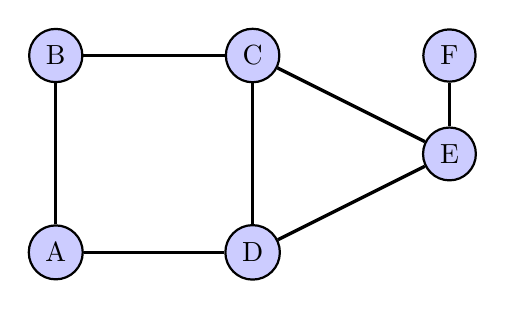
\begin{tikzpicture}[baseline=(A)]
    \begin{scope}[every node/.style={fill=blue!20,circle,thick,draw}]
        \node (A) at (0,0) {A};
        \node (B) at (0,2.5) {B};
        \node (C) at (2.5,2.5) {C};
        \node (D) at (2.5,0) {D};
        \node (E) at (5,1.25) {E};
        \node (F) at (5,2.5) {F} ;
    \end{scope}
    
    \begin{scope}[>={Stealth[black]},
                  every node/.style={fill=white,circle},
                  every edge/.style={draw=black,very thick}]
        \path [-] (A) edge (B);
        \path [-] (B) edge (C);
        \path [-] (A) edge (D);
        \path [-] (D) edge (C);
        \path [-] (D) edge (E);
        \path [-] (C) edge (E);
        \path [-] (E) edge (F); 
    
    \end{scope}
\end{tikzpicture}
\quad
\quad
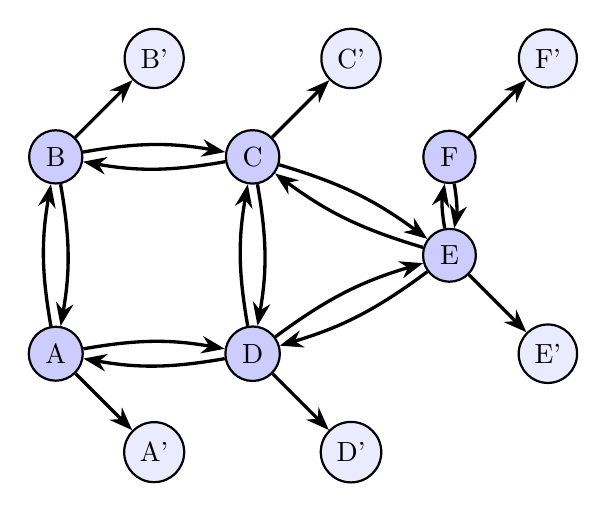
\begin{tikzpicture}[baseline= (A)]
    \begin{scope}[every node/.style={fill= blue!20, circle,thick,draw}]
        \node (A) at (0,0) {A};
        \node (B) at (0,2.5) {B};
        \node (C) at (2.5,2.5) {C};
        \node (D) at (2.5,0) {D};
        \node (E) at (5,1.25) {E};
        \node (F) at (5,2.5) {F} ;
    \end{scope}
    
    \begin{scope}[every node/.style={fill= blue!8, circle,thick,draw}]
        \node (A') at (1.25,-1.25) {A'};
        \node (B') at (1.25,3.75) {B'};
        \node (C') at (3.75,3.75) {C'};
        \node (D') at (3.75,-1.25) {D'};
        \node (E') at (6.25,0) {E'};
        \node (F') at (6.25,3.75) {F'} ;
    \end{scope}
    
    \begin{scope}[>={Stealth[black]},
                  every node/.style={fill=white,circle},
                  every edge/.style={draw=black,very thick}]
        \path [->,bend left=10] (D) edge (C);
        \path [->,bend left=10] (C) edge (D);
        \path [->,bend left=10] (A) edge (B);
        \path [->,bend left=10] (B) edge (A);
        \path [->,bend left=10] (B) edge (C);
        \path [->,bend left=10] (C) edge (B);
        \path [->,bend left=10] (A) edge (D);
        \path [->,bend left=10] (D) edge (E);
        \path [->,bend left=10] (E) edge (D);
        \path [->,bend left=10] (C) edge (E);
        \path [->,bend left=10] (E) edge (C);
        \path [->,bend left=10] (E) edge (F);
        \path [->,bend left=10] (F) edge (E);
        \path [->,bend left=10] (D) edge (A);
        \path [->] (A) edge (A');
        \path [->] (B) edge (B');
        \path [->] (C) edge (C');
        \path [->] (D) edge (D');
        \path [->] (E) edge (E');
        \path [->] (F) edge (F');
    
    \end{scope}
\end{tikzpicture}
}
\caption{Pretvorba grafa $G$ v digraf $B(G)$.} \label{fig:M1}
\end{figure}

Iz vsakega vozlišča na zgornjem digrafu gre do sosednjih vozlišč in pripadajočega končnega vozlišča le po ena usmerjena povezava, saj je možnost premika evra za vsak scenarij enaka. Tako velja, da bo število žetonov v končnem vozlišču po koncu algoritma enako številu izstrelitev iz vozlišča, ki je z njim povezano.
Poleg tega velja, da ima vsako vozlišče v kritični razporeditvi toliko žetonov, kot ima sosedov v grafu sosednosti $G$.

Ko graf sosednosti $G$ prevedemo na ustrezen digraf $B(G)$, določimo začetnega imetnika evra in izvedemo Engelov algoritem. Verjetnost zmage poljubnega posameznika je tako enaka
$$
\text{verjetnost zmage $i$-tega igralca} = \frac{\text{število žetonov v končnem vozlišču $i$-tega igralca}}{\text{število vseh dodanih žetonov}} \ .
$$

S stohastičnim abakusom lahko torej na preprost način določimo iskane verjetnosti za različne grafe sosednosti. 
Zanima nas še, kdaj se igra konča. Z drugimi besedami, zanima nas, kolikšno je pričakovano število potez preden eden
od igralcev evro osvoji. Engelov algoritem tudi v tem primeru nudi preprosto in elegantno rešitev. Opazujemo, kako 
hitro se žetoni premikajo v končna vozlišča. Ob izvajanju algoritma v digraf skupno dodamo neko število žetonov, 
ki ga bomo označili s $c$. Med postopkom izstreljujemo žetone iz vozlišč in ob tem povzročamo premike na naslednji način: ko eno od 
vozlišč z $d$ sosedi (oz.\,\,$d+1$ sosedi v digrafu) izstreli žetone, s tem povzroči $d+1$ premikov. skupno število vseh premikov bomo označili z $m$.
Tako je pričakovano število potez, preden žeton doseže katero koli končno vozlišče, enako $\frac{m}{c}$, saj velja, 
da v $m$ potezah $c$ žetonov pride do končnih vozlišč. Pričakovana trajanje igre je torej enako $\frac{m}{c}$ potez.


Pomembno se je zavedati, da je Engelov algoritem le eden od možnih načinov reševanja zgornjega problema. Z drugimi pristopi 
bi do odgovorov lahko prišli mnogo hitreje, saj je postopek izstrelitev žetonov precej zamuden za veliko število vozlišč.
Kljub temu je uporaba stohastičnega abakusa v igrah podajanja evra smiselna, saj gre za preprost in splošno dojemljiv algoritem, 
ki za svoje izvajanje ne zahteva globjega matematičnega predznanja. Poleg tega so nekatere lastnosti, ki se ob tovrstnih igrah 
pojavljajo in jih bomo omenili v nadaljevanju, na ta način bolj jasno razvidne.



\section{Graf poti na $n$ vozliščih}

Postavitve igralcev v igri podajanja evra so lahko zelo različne, za začetek pa se bomo osredotočili na igro, kjer igralci stojijo v ravni vrsti. Primer je zanimiv zaradi povezave med verjetnostjo zmage posameznika in Fibonaccijevimi števili. 
Opazovali bomo dogajanje med izvajanjem Engelovega algoritma na grafu sosednosti $P_n$, kjer začetni igralec stoji najbolj levo oz.\,\,najbolj desno v vrsti. Stohastični abakus se na
grafu takšne oblike izvede na digrafu $B(P_{n})$, ki je na sliki \ref{fig:M2} prikazan za pot s petimi vozlišči. Digraf je prikazan v začetnem stanju s kritično razporeditvijo žetonov in v stanju po končanem algoritmu z ustreznim številom žetonov v končnih vozliščih.

\begin{figure}[t]
        \centering
        \fbox{
        
        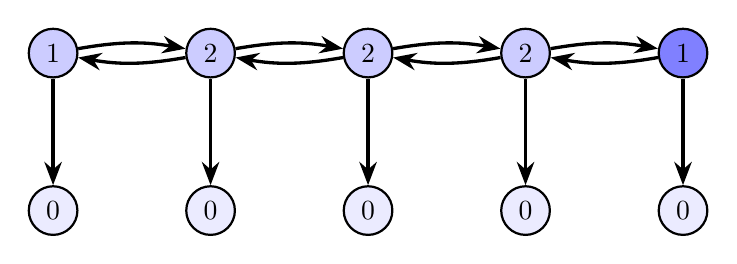
\begin{tikzpicture}
            \begin{scope}[every node/.style={fill= blue!20, circle,thick,draw}]
                \node (A) at (0,0) {1};
                \node (B) at (2,0) {2};
                \node (C) at (4,0) {2};
                \node (D) at (6,0) {2};
                \node (E) [fill=blue!50] at (8,0) {1};
                
            \end{scope}
            
            \begin{scope}[every node/.style={fill= blue!8, circle,thick,draw}]
                \node (A') at (0,-2) {0};
                \node (B') at (2,-2) {0};
                \node (C') at (4,-2) {0};
                \node (D') at (6,-2) {0};
                \node (E') at (8,-2) {0};
                
            \end{scope}
            
            \begin{scope}[>={Stealth[black]},
                          every node/.style={fill=white,circle},
                          every edge/.style={draw=black,very thick}]
                \path [->,bend left=10] (D) edge (C);
                \path [->,bend left=10] (C) edge (D);
                \path [->,bend left=10] (A) edge (B);
                \path [->,bend left=10] (B) edge (A);
                \path [->,bend left=10] (B) edge (C);
                \path [->,bend left=10] (C) edge (B);
                \path [->,bend left=10] (D) edge (E);
                \path [->,bend left=10] (E) edge (D);
                \path [->] (A) edge (A');
                \path [->] (B) edge (B');
                \path [->] (C) edge (C');
                \path [->] (D) edge (D');
                \path [->] (E) edge (E');
            
            \end{scope}
        \end{tikzpicture}
        }
        %
        \bigskip

        \fbox{

        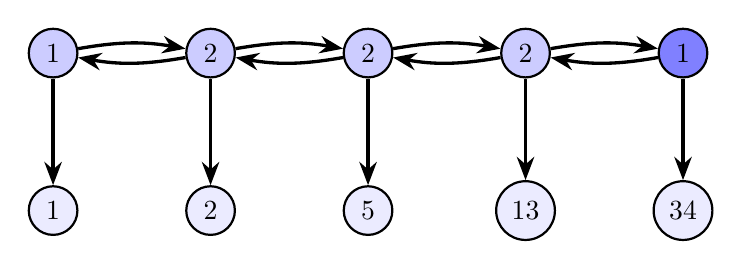
\begin{tikzpicture}
            \begin{scope}[every node/.style={fill= blue!20, circle,thick,draw}]
                \node (A) at (0,0) {1};
                \node (B) at (2,0) {2};
                \node (C) at (4,0) {2};
                \node (D) at (6,0) {2};
                \node (E) [fill=blue!50] at (8,0) {1};
                
            \end{scope}
            
                        
            \begin{scope}[every node/.style={fill= blue!8, circle,thick,draw}]
                \node (A') at (0,-2) {1};
                \node (B') at (2,-2) {2};
                \node (C') at (4,-2) {5};
                \node (D') at (6,-2) {13};
                \node (E') at (8,-2) {34};
                
            \end{scope}
            
            \begin{scope}[>={Stealth[black]},
                          every node/.style={fill=white,circle},
                          every edge/.style={draw=black,very thick}]
                \path [->,bend left=10] (D) edge (C);
                \path [->,bend left=10] (C) edge (D);
                \path [->,bend left=10] (A) edge (B);
                \path [->,bend left=10] (B) edge (A);
                \path [->,bend left=10] (B) edge (C);
                \path [->,bend left=10] (C) edge (B);
                \path [->,bend left=10] (D) edge (E);
                \path [->,bend left=10] (E) edge (D);
                \path [->] (A) edge (A');
                \path [->] (B) edge (B');
                \path [->] (C) edge (C');
                \path [->] (D) edge (D');
                \path [->] (E) edge (E');
            
            \end{scope}
        \end{tikzpicture}
        }
        \caption{Primer izvedbe stohastičnega abakusa na grafu poti.} \label{fig:M2}
        \end{figure}


\begin{izrek}\label{Izrek 1}
Recimo, da opazujemo igro podajanja evra z $n$ igralci razporejenimi v graf poti $P_{n}$. Njihove položaje označimo z indeksi od $1$ do $n$, začetni imetnik evra pa naj bo igralec na mestu $n$. Po izvedbi Engelovega algoritma na digrafu $B(P_{n})$ je število žetonov v končnih vozliščih pripadajočih notranjih vozlišč, z indeksi od $1$ do $n$, po vrsti
enako $f_1, f_3, f_5, \ldots, f_{2n-1}$. Torej je verjetnost zmage igralca na poziciji $k$ enaka $\frac{f_{2k-1}}{f_{2n}}$.
\end{izrek}

\begin{dokaz}
V prvem koraku je potrebno dokazati, da je imenovalec v zadnjem ulomku res enak seštevku vseh žetonov v končnih vozliščih. 
Radi bi torej dokazali enakost $f_1+f_3+f_5+\ldots+f_{2n-1}=f_{2n}$, pri čemer bomo uporabili preprosto indukcijo.
\begin{itemize}
    \item [] \textbf{Baza indukcije:} \quad $1=f_1=f_2=1$
    \item [] \textbf{Indukcijski korak:} \quad $f_1+f_3+f_5+\ldots+f_{2n-1}+f_{2n+1} = f_{2n} + f_{2n+1} = f_{2n+2}$ \\
    Pri izračunu smo pri prvi enakosti uporabili indukcijsko predpostavko, pri drugi pa definicijo Fibonaccijevih števil.
\end{itemize}

\noindent V drugem koraku je potrebno dokazati še, da so števila žetonov v končnih vozliščih res zaporedni lihi členi
Fibonaccijevega zaporedja. Pri tem bomo upoštevali dejstvo, da je vrstni red v katerem izstreljujemo žetone irelevanten za končni izid algoritma.
Tudi tokrat rezultat dokazujemo z indukcijo.
\begin{itemize}
    \item [] \textbf{Baza indukcije:} Dokaz za pot z enim vozliščem $P_1$ je očiten.
    % Ko dodamo žeton na edino vozlišče, ki je v kritičnem stanju prazno, se to sproži in pošlje žeton v terminalno vozlišče, pri tem pa samo ostane v kritično polnem stanju. Tako je število žetonov v kritičnem vozlišču po izvedenem Englovem algoritmu enako $1=f_1$.
    \item [] \textbf{Indukcijski korak:} Predpostavimo, da je število žetonov v končnih vozliščih po izvedenem algoritmu na 
    digrafu $B(P_{n})$ res enako $f_{2k-1}$ za vsako notranje vozlišče z indeksom $1\le k\le n$. 
    Sedaj opazujemo algoritem na digrafu $B(P_{n+1})$, kjer je začetno vozlišče indeksirano z $n+1$. Sestavili bomo strategijo, 
    ki bo zaključila Engelov algoritem na omenjenem digrafu. Ob začetku je torej sistem v kritični razporeditvi.
    V začetno vozlišče z indeksom $n+1$ položimo $2\cdot f_{2n}$ žetonov, pri čemer žetone iz tega vozlišča izstrelimo $f_{2n}$-krat in 
    po koncu ostane v kritičnem stanju. Pri tem se $f_{2n}$ žetonov pomakne v vozlišče z indeksom $n$ in $f_{2n}$ žetonov v končno vozlišče začetnega vozlišča.
    Sedaj opazujemo dogajanje, ki ga sproži $f_{2n}$ novih žetonov v vozlišču $n$. Po predpostavki vemo, da bi za izvedbo Engelovega algoritma na $B(P_{n})$ potrebovali $f_{2n}$ žetonov, pri čemer bi žetone iz vozlišča $n$ izstrelili $f_{2n-1}$-krat. 
    Ko prvi žeton prispe v vozlišče $n$, njegove žetone izstrelimo in pošljemo po en žeton v končno vozlišče, vozlišče z indeksom $n-1$ in vozlišče z indeksom $n+1$. Žetone iz vozlišča $n+1$ po dodanem žetonu izstrelimo, s čimer se en žeton spet vrne v vozlišče $n$.
    V vozlišče $n+1$ po koncu dodamo še en žeton, da ga pustimo v kritični razporeditvi. Torej vsakič, ko bomo izstrelili vozlišče $n$, bomo v sistem dodali še en dodaten žeton, pri tem pa se bo povečalo tudi število žetonov v končnem vozlišču začetnega vozlišča.
    Zanima nas torej, kolikokrat bomo vozlišče $n$ izstrelili. Če bi bilo krajišče robno, bi iz predpostavke vedeli, da ga bomo izstrelili natanko $f_{2n-1}$-krat. Ob dodanem vozlišču na desni strani se poveča število sosedov za ena, torej ima v kritični razporeditvi en žeton več kot prej.
    Vemo, da se ob vsaki izstrelitvi ob zgoraj opisanem postopku en žeton vrne v vozlišče, kar izniči vpliv dodatnega soseda pri številu izstrelitev. Za vsako novo izstrelitev je namreč treba dodati isto število novih žetonov, torej vozlišče $n$ tudi v tem primeru izstrelimo $f_{2n-1}$-krat.
    Situacija se prevede na Engelov algoritem na $B(P_n)$, pri čemer so števila žetonov v končnih vozliščih vozlišč z indeksi od $1$ do $n$ po vrsti enaka $f_1,f_3,f_5,\ldots,f_{2n-1}$. V sistem smo skupno dodali $2\cdot f_{2n}+ f_{2n-1} = f_{2n+2}$ žetonov, pri čemer je bilo število
    izstrelitev začetnega vozlišča enako $f_{2n}+f_{2n-1}=f_{2n+1}$.
    
    

\end{itemize}
\hfill \QED

 
    
\end{dokaz}

Igra podajanja evra v zgoraj opisani situaciji torej porodi povezavo z lihimi členi Fibonaccijevega zaporedja. Iz izreka je razvidno, da je verjetnost zmage začetnega igralca enaka $\frac{f_{2n-1}}{f_{2n}}$, torej gre za razmerje dveh zaporednih Fibonaccijevih števil. Če bomo število igralcev povečevali čez vse meje,
bo tako verjetnost zmage začetnega igralca enaka $\frac{1}{\phi}$, kjer je $\phi$ razmerje zlatega reza.

Pričakovano število potez v igri je, kot smo že prej razmislili, enako $\frac{m}{c}$. Pri izvedbi Engelovega algoritma smo v začetno vozlišče dodali $f_{2n}$ novih žetonov, torej je $c=f_{2n}$, seštevek vseh premikov žetonov pa je za $n \ge 3$ enak
\begin{align*}
    m &= 2f_1+3(f_3+f_5+\ldots+f_{2n-3}) + 2f_{2n-1} \\
    &=2\sum_{i=1}^{n}f_{2i-1} + \sum_{i=2}^{n-1}f_{2i-1} \\
    &=2f_{2n} + (f_{2n-2}-1) \ .
\end{align*}

Pri izračunu smo pri prvem enačaju upoštevali dejstvo, da je število žetonov v končnem vozlišču po izvedbi algoritma enako številu izstrelitev pripadajočega notranjega vozlišča, robni vozlišči imata dva soseda, ostala vozlišča pa imajo tri sosede, pri tretjem enačaju pa smo uporabili ravnokar dokazano formulo iz izreka \ref{Izrek 1}.
Pričakovano število potez v igri je torej za poljubno število igralcev $n\ge3$ enako 
$$
\frac{2f_{2n} + (f_{2n-2}-1)}{f_{2n}} \ .
$$

Zanimivo je tudi opazovati dogajanje pri malenkost spremenjeni igri. Naj velja, da če evro pride 
do zadnjega igralca (oz.\,\,v našem primeru igralca z indeksom $1$), ta avtomatično zmaga. Digraf za izvedbo Engelovega algoritma je v novi igri enak, 
sprememba je le v tem, da od vozlišča z indeksom $1$ tokrat ni usmerjene povezave do vozlišča z indeksom $2$. 
Izkaže se, da so števila žetonov v končnih vozliščih, ki po vrsti pripadajo vozliščem z indeksi od $1$ 
do $n$, enaka $f_1,f_2,f_4,f_6,\ldots,f_{2n-2}$.
Število žetonov potrebnih za izvedbo Engelovega algoritma pa je v tem primeru enako $f_1+f_2+f_4+\ldots+f_{2n-2}=f_{2n-1}$, 
kar ponovno implicira, da je verjetnost zmage začetnega igralca ob neskončno članih igre enaka $\frac{1}{\phi}$. 
Torej v opisani igri opazimo povezavo s sodimi členi Fibonaccijevega zaporedja (z izjemo prvega člena), 
kar bi dokazali na podoben način kot prejšnji izrek.
Verjetnost zmage posameznega igralca je za vsakega, razen za zadnjega, večja v prvi različici igre, hkrati pa velja, da igra takrat traja dlje.
Če si namreč pogledamo pričakovano število potez, je to enako
\begin{align*}
    \frac{m}{c} &= \frac{2f_1 + 3(f_2+f_4+\ldots+f_{2n-4})+ 2f_{2n-2}}{f_{2n-1}} \\
    &= \frac{2f_{2n-1} + (f_{2n-3}-1)}{f_{2n-1}} \ ,
\end{align*}
kar je manj kot v prvotni različici igre (neenakost lahko dokažemo z indukcijo).
%\subsection{Graf poti na $n$ točkah z začetkom v notranjem vozlišču}

\section{Randomizirane igre podajanja evra}
Igro podajanja evra smo predstavili na eni najbolj preprostih formacij igralcev, s katero si lahko pomagamo priti do rezultatov na bolj kompleksnih grafih sosednosti. 
S tem se v članku ne bomo podrobneje ukvarjali, pogledali pa si bomo igro, v kateri vpeljemo še eno slučajno spremenljivko, ki bo predstavljala naključno izbiro začetnega igralca. Takim
igram pravimo \emph{randomizirane} igre podajanja evra. Opazovali bomo poljubno formacijo igralcev in ugotavljali, kako modificirana igra vpliva na verjetnost zmage vsakega posameznika. 

Da bomo lahko na randomizirani igri z grafom sosednosti $G$ uporabili pristop s stohastičnim abakusom, moramo igro modelirati z ustreznim digrafom, ki ga bomo označevali z $D(G)$.
Digraf konstruiramo tako, da iz prvotnega grafa najprej na enak način kot prej izpeljemo digraf $B(G)$ in nato dodamo dodatno vozlišče, iz katerega gredo usmerjene povezave do vsakega izmed notranjih vozlišč. 
S tem predstavimo faktor naključne izbire prvega igralca, saj gre do vsakega vozlišča točno ena povezava, kar odraža dejstvo, da ob $n$ 
igralcih vsak začne z enako verjetnostjo $\frac{1}{n}$. Novo vozlišče je tudi začetno vozlišče, torej vanj dodajamo nove žetone ob izvajanju Engelovega algoritma.

Smiselno vprašanje, ki si ga igralec ob začetku katere koli igre podajanja evra postavi, je, kateri položaj v formaciji mu bo z največjo verjetnostjo prinesel dobiček. V primeru poti je bilo glede na dokazani izrek bolje, da zavzame pozicijo čim bližje začetnemu igralcu.
V randomizirani igri pa je situacija drugačna. Poglejmo si enak primer kot prej, torej pot na petih vozliščih, kjer je izbira začetnega igralca naključna. Digraf je na začetku v kritični razporeditvi.
Ko izstrelimo žetone iz začetnega vozlišča, takoj zatem izstrelimo žetone tudi iz vseh notranjih vozlišč. Pri tem se število žetonov v končnih vozliščih poveča na 1, notranja vozlišča pa so spet v kritični razporeditvi. Na začetno vozlišče položimo 5 novih žetonov, s čimer je Engelov algoritem zaključen (glej sliko \ref{fig:M3}).
Torej je izbira pozicije v igri nepomembna, saj ima vsak igralec enake možnosti za zmago. Tudi algoritem je v tem primeru veliko hitrejši, saj je potrebno dodati le pet novih žetonov, pri čemer jih je bilo prej potrebno dodati $47$. Izkaže se, da ugotovitev velja za poljuben graf sosednosti $G$.


\begin{figure}[t]
    \centering
    \fbox{
    
    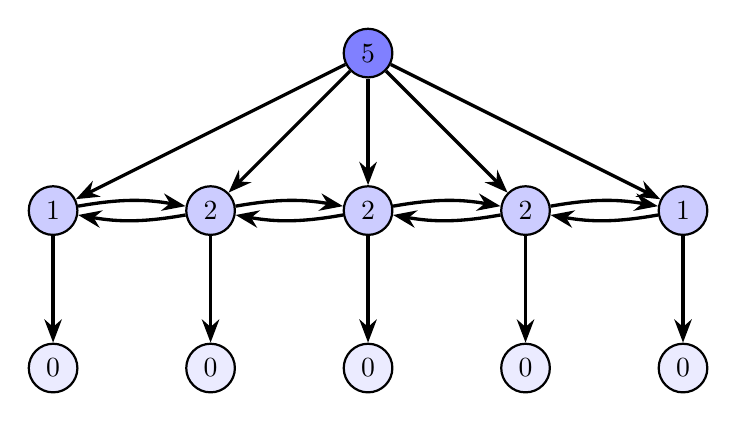
\begin{tikzpicture}
        \begin{scope}[every node/.style={fill= blue!20, circle,thick,draw}]
            \node (A) at (0,0) {1};
            \node (B) at (2,0) {2};
            \node (C) at (4,0) {2};
            \node (D) at (6,0) {2};
            \node (E) at (8,0) {1};
            \node (F) [fill=blue!50] at (4,2) {5};

        \end{scope}
        
        \begin{scope}[every node/.style={fill= blue!8, circle,thick,draw}]
            \node (A') at (0,-2) {0};
            \node (B') at (2,-2) {0};
            \node (C') at (4,-2) {0};
            \node (D') at (6,-2) {0};
            \node (E') at (8,-2) {0};
            
            
        \end{scope}
        
        \begin{scope}[>={Stealth[black]},
                      every node/.style={fill=white,circle},
                      every edge/.style={draw=black,very thick}]
            \path [->,bend left=10] (D) edge (C);
            \path [->,bend left=10] (C) edge (D);
            \path [->,bend left=10] (A) edge (B);
            \path [->,bend left=10] (B) edge (A);
            \path [->,bend left=10] (B) edge (C);
            \path [->,bend left=10] (C) edge (B);
            \path [->,bend left=10] (D) edge (E);
            \path [->,bend left=10] (E) edge (D);
            \path [->] (A) edge (A');
            \path [->] (B) edge (B');
            \path [->] (C) edge (C');
            \path [->] (D) edge (D');
            \path [->] (E) edge (E');
            \path [->] (F) edge (A);
            \path [->] (F) edge (B);
            \path [->] (F) edge (C);
            \path [->] (F) edge (D);
            \path [->] (F) edge (E);
        
        \end{scope}
    \end{tikzpicture}
    }
    %
    \bigskip

    \fbox{

    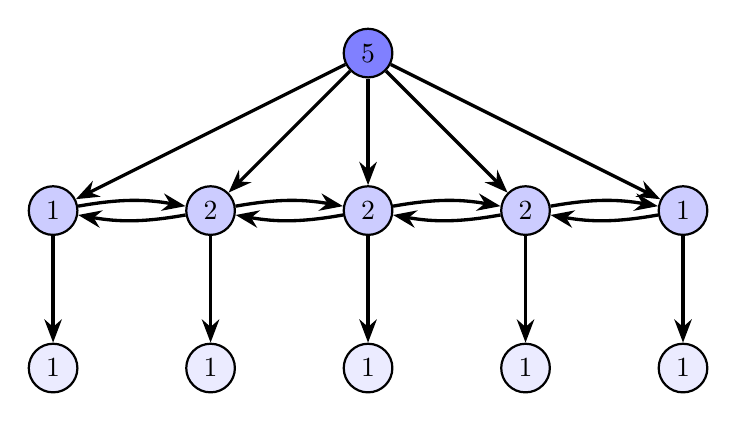
\begin{tikzpicture}
        \begin{scope}[every node/.style={fill= blue!20, circle,thick,draw}]
            \node (A) at (0,0) {1};
            \node (B) at (2,0) {2};
            \node (C) at (4,0) {2};
            \node (D) at (6,0) {2};
            \node (E) at (8,0) {1};
            \node (F) [fill=blue!50] at (4,2) {5};
            
        \end{scope}
        
                    
        \begin{scope}[every node/.style={fill= blue!8, circle,thick,draw}]
            \node (A') at (0,-2) {1};
            \node (B') at (2,-2) {1};
            \node (C') at (4,-2) {1};
            \node (D') at (6,-2) {1};
            \node (E') at (8,-2) {1};
            
        \end{scope}
        
        \begin{scope}[>={Stealth[black]},
                      every node/.style={fill=white,circle},
                      every edge/.style={draw=black,very thick}]
            \path [->,bend left=10] (D) edge (C);
            \path [->,bend left=10] (C) edge (D);
            \path [->,bend left=10] (A) edge (B);
            \path [->,bend left=10] (B) edge (A);
            \path [->,bend left=10] (B) edge (C);
            \path [->,bend left=10] (C) edge (B);
            \path [->,bend left=10] (D) edge (E);
            \path [->,bend left=10] (E) edge (D);
            \path [->] (A) edge (A');
            \path [->] (B) edge (B');
            \path [->] (C) edge (C');
            \path [->] (D) edge (D');
            \path [->] (E) edge (E');
            \path [->] (F) edge (A);
            \path [->] (F) edge (B);
            \path [->] (F) edge (C);
            \path [->] (F) edge (D);
            \path [->] (F) edge (E);
        
        \end{scope}
    \end{tikzpicture}
    }
    \caption{Randomizirana igra podajanja evra na grafu $P_{5}$} \label{fig:M3}
    \end{figure}


\begin{izrek}
    Randomizirana igra podajanja evra je poštena za vse grafe sosednosti $G$. To pomeni, da ima v igri z $n$ igralci ne glede na postavitev vsak igralec enako verjetnost za zmago.
\end{izrek}

\begin{dokaz}
   Opazujemo poljubno igro podajanja evra modelirano z grafom sosednosti $G(V,E)$ z \newline 
   $|V|=n$. Vozlišča označimo z $v_1,v_2,\ldots,v_n$. 
   Recimo, da graf ne vsebuje nobene povezave.
   Da iz $G$ konstruiramo ustrezen digraf $D(G)$ za randomizirano igro, dodamo $n$ končnih vozlišč, eno novo vozlišče $s$ ter usmerjene povezave od $s$ do $v_i$, za vsak $ i\in {1,2,\ldots,n}$.
   Digraf $D(G)$ ima kritično razporeditev, ko $s$ vsebuje $n$, ostala vozlišča pa nič žetonov. V $s$ dodamo $n$ novih žetonov, pri čemer iz njega izstrelimo žetone in nato obmiruje v kritični razporeditvi.
   Ob tem se ob pridobljenih novih žetonih sprožijo tudi vozlišča $v_1,v_2,\ldots,v_n$, pri čemer se vsako končno vozlišče napolni za en žeton, digraf pa je spet v kritični razporeditvi.
   V tem primeru očitno velja, da je verjetnost zmage vsakega igralca enaka $\frac{1}{n}$.

   Pri dokazovanju izreka na grafu s poljubnim smiselnim številom povezav uporabimo naslednji razmislek: če na digraf $G$ dodamo povezavo $v_kv_j$, bosta torej na grafu $D(G)$ dve novi usmerjeni povezavi med vozliščema $v_k$ in $v_j$.
   Ko iz teh dveh vozlišč izstrelimo žetone, bosta zaradi novega odnosa sosednosti obe izstrelili po en žeton več, hkrati pa bosta en žeton več tudi prejeli. Podobno kot prej v $s$ dodamo $n$ novih žetonov, pri čemer iz njega izstrelimo žetone in nato obmiruje v kritični razporeditvi.
   Ob tem se ob pridobljenih novih žetonih sprožijo tudi vozlišča $v_1,v_2,\ldots,v_n$. Za vsako vozlišče $v_i, i\in{1,2,\ldots,n}$ velja, da en žeton pošlje v svoje končno vozlišče, po en žeton pošlje vsakemu svojemu sosedu, hkrati pa tudi prejme po en žeton od vsakega izmed njih.
   Torej se število žetonov na vozlišču ne spremeni, sistem pa je tako spet v kritični razporeditvi.
   \hfill \QED

\end{dokaz}

Poglejmo si še, kako je s pričakovanim številom potez za randomizirano igro z grafom sosednosti $G(V,E)$ z $|V|=n$ in $|E|=e$. Skupno število dodanih žetonov ob izvedbi Engelovega algoritma 
je po prejšnjem razmisleku enako $n$, skupno število premikov pa je enako $2n+2e$. Začetno vozlišče se namreč sproži natanko enkrat, kar povzroči $n$ premikov, 
prav tako pa se natanko enkrat sprožijo tudi vsa notranja vozlišča. 
Ob tem se na grafu zgodi $n$ premikov, ko se po en žeton premakne v ustrezno končno vozlišče, in še $2e$ premikov po ostalih usmerjenih povezavah. 

\section{Zaključek}
Predstavili smo Engelov stohastični abakus in s pomočjo iger podajanja evra pokazali preprostost in elegantnost rešitve določenih problemov z njegovo uporabo. 
Odkrili smo povezavo med stohastičnim abakusom in Fibonaccijevimi števili, zaintresiran bralec lahko še več podobnih povezav najde v \cite{torr}. To ni edini, način s katerim se lahko lotimo takšnih problemov, elegantno jih lahko rešimo na primer tudi s pomočjo harmoničnih funkcij.


\begin{thebibliography}{99}

\bibitem{torr} Bruce Torrence, \emph{  Passing the Buck and Firing Fibonacci: Adventures with the Stochastic Abacus}, The American Mathematical Monthly , MAY 2019, Vol. 126, No. 5 (MAY 2019), pp. 387-399.
\bibitem{snell} J. Laurie Snell, \emph{The Engel algorithm for absorbing Markov chains}, [Dostopano dne 16. 2. 2024], Spletna stran: https://math.dartmouth.edu/~doyle/docs/engel/engel.pdf. 
\bibitem{eng} Arthur Engel, \emph{Why Does the Probabilistic Abacus Work?},  Educational Studies in Mathematics, Vol. 7, No. 1/2 (Jul., 1976), pp. 59-69. 
\bibitem{ver} Janez Bernik, \emph{Verjetnost 2, 1.del; Markovske verige v diskretnem času}.

\end{thebibliography}







\end{document}